\section{Gruppen}

\begin{definition}\label{def:gruppe}
    Sei $\mathfrak{G} = (G, \cdot, e, {}^{-1})$ eine Gruppe.
    \begin{itemize}
        \item Wir nennen $|G|$ die \emph{Ordnung} der Gruppe.\index{Gruppe!Ordnung}
        \item Sei $g \in G$, so erzeugt dieses Element eine Untergruppe
        $$ \langle \{ g \} \rangle = \{ g^n \mid n \in \mathbb{Z} \}. $$
        Wir nennen $|\langle\{g\}\rangle|$ die \emph{Ordnung} von $g$ und schreiben auch $\ord(g)$. Ist $\ord(g)$ endlich, so heißt $g$ \emph{Torsionselement}.\index{Gruppe!Torsionselement}
        \item $\mathfrak{G}$ heißt \emph{zyklisch}, falls es ein $g \in G$ mit $G = \langle\{g\}\rangle$ gibt.\index{Gruppe!zyklisch}
    \end{itemize}
\end{definition}

\begin{remark}
    Im Folgenden werden wir Gruppen durch ihre Trägermengen identifizieren. Für die Gruppe $\mathfrak{G} = (G, \cdot, e, {}^{-1})$ wird oft nur $G$ geschrieben.
\end{remark}

\begin{example} {\ }
    \begin{enumerate}
        \item Betrachte $\mathbb{Z} \times \mathbb{Z}_m$, so ist $\ord(1,0) = \infty$ und $\ord(0,1) = m$.
        \item Betrachte $\mathbb{Z}_6$, so ist $\ord(1) = 6$, $\ord(2) = 3$ und $\ord(3) = 2$.
    \end{enumerate}
\end{example}

\begin{example} {\ }
    \begin{enumerate}
        \item Die Gruppen $(\mathbb{Z}, +, 0, -) = \langle\{1\}\rangle, (\mathbb{Z}_m, +, 0, -) = \langle\{1\}\rangle$ sind zyklisch.
        \item Die Gruppe $(\Gl_2(\mathbb{Q}), \cdot, E_2, {}^{-1})$ ist \emph{nicht} zyklisch, da -- wie wir noch sehen werden -- zyklische Gruppen abelsch sind.
    \end{enumerate}
\end{example}

\notedate{30.03.2023}

\subsection{Nebenklassen und Normalteiler}

\begin{definition}
    Seien $G$ eine Gruppe, $U \le G$ eine Untergruppe und $g \in G$. Wir definieren 
    \begin{itemize}
        \item die \emph{Linksnebenklasse von $g$ nach $U$}\index{Linksnebenklasse} $gU := \{gu \mid u \in U\}$ und
        \item die \emph{Rechtsnebenklasse von $g$ nach $U$}\index{Rechtsnebenklasse} $Ug := \{ug \mid u \in U\}$.
    \end{itemize}
\end{definition}

\begin{lemma}\label{lemma:euqivrel_linksnebenklassen}
    Seien $G$ eine Gruppe, $U \le G$ eine Untergruppe und $g, g', x, y \in G$. Dann gilt:
    \begin{enumerate}
        \item Die Menge $\{gU \mid g \in G\}$ aller Linksnebenklassen von $g$ nach $U$ bildet eine Partition von $G$.
        \item Es gilt $gU = g'U$ genau dann, wenn $g^{-1}g' \in U$.
        \item Die Partition induziert eine Äquivalenzrelation $\sim$ auf $G$, wobei $x \sim y \Leftrightarrow \exists \tilde{g} \in G: x,y \in \tilde{g}U$.
        \item Es gilt für diese Äquivalenzrelation $x \sim y \Leftrightarrow x^{-1}y \in U$.\label{item:lemma:euqivrel_linksnebenklassen_4}
        \item Es ist $U = [e]_{\sim}$.
    \end{enumerate}
    
\end{lemma}
\begin{proof}{\ }
    \begin{enumerate}
        \item Es gilt $G = \bigcup_{g \in G} gU$, denn für $h \in G$ ist $h \in hU$, weil $e \in U$ und $h = h \cdot e$ ist. 
        
        Es bleibt noch zu zeigen, dass die Nebenklassen disjunkt sind. Dafür zeigen wir, dass nicht disjunkte Linksnebenklassen gleich sind. Seien also $g, g' \in G$ beliebig mit $gU \cap g'U \not= \emptyset$. Es existieren dann $u, u' \in U$, sodass $g u = g' u'$. Sei $a = g  u_a \in gU$ beliebig. Es ist dann $$ a = g u_a = g u u^{-1} u_a = g' \underbrace{u' u^{-1} u_a}_{\in U} \in g'U, $$
        also $gU \subseteq g'U$. Analog erhält man die andere Mengeninklusion, womit $gU = g'U$ gilt.
        \item Es ist 
        $$gU = g'U \;\Leftrightarrow\; \exists u, u' \in U: gu = g'u' \;\Leftrightarrow\; \exists u, u' \in U: u\left(u'\right)^{-1} = g^{-1}g' \;\Leftrightarrow\; g^{-1}g' \in U.$$
        \item Klarerweise wird durch eine Partition eine Äquivalenzrelation induziert. $\exists \tilde{g} \in G: x,y \in \tilde{g}U$ ist äquivalent dazu, dass $xU = yU$, was wiederum äquivalent dazu ist, dass $x, y$ die gleiche Äquivalenzklasse haben.
        \item \begin{itemize}[leftmargin=1cm]
            \item[``$\Rightarrow$'':] Es gibt $u, u' \in U$, sodass $x = g u$ und $y = g u'$. Es ist also $x^{-1} y = u^{-1} g^{-1} \cdot g  u' = u^{-1} u' \in U$.
            \item[``$\Leftarrow$'':] Es gilt $x^{-1}\cdot y = u$, also $y = x\cdot u$.  Es ist nun $x \in xU$ und auch  $y \in xU$, also $x \sim y$. 
        \end{itemize}
        \item Es ist $a \in [e]_\sim \;\Leftrightarrow\; e \sim a \;\Leftrightarrow\; e^{-1} a = a \in U $.
    \end{enumerate}
\end{proof}

\begin{remark}
    \cref{lemma:euqivrel_linksnebenklassen} gilt analog für Rechtsnebenklassen. Im Allgemeinen erhält man dabei allerdings eine andere Äquivalenzrelation.
\end{remark}

\begin{lemma}
    Seien $G$ eine Gruppe, $U \le G$ eine Untergruppe und $g \in G$. Es gilt $$\vert gU \vert = \vert U \vert = \vert Ug \vert.$$
\end{lemma}
\begin{proof}
    Definieren wir die Funktion $\varphi: U \to gU, u \mapsto g\cdot u$ und zeigen, dass sie bijektiv ist. Die Surjektivität ist klar, da $gU$ genau als das Bild von $\varphi$ definiert ist. Die Injektivität erhalten wir wegen $gu = gu' \Rightarrow u = u'$. Damit ist $\vert U \vert = \vert gU \vert$. Die zweite Gleichheit wird analog gezeigt.
\end{proof}

\begin{remark}\label{rem:nebenklassenzerlegung_endlich}
    Ist $G$ eine endliche Gruppe, dann gilt $\vert G \vert = \vert \{gU \mid g \in G\} \vert \cdot \vert U \vert$, da alle Links-/Rechtsnebenklassen gleich mächtig sind. Durch umformen zu $\vert \{gU \mid g \in G\} \vert = \frac{\vert G \vert}{\vert U \vert}$ erhalten wir, dass es gleich viele Linksnebenklassen wie Rechtsnebenklassen gibt.

    \begin{figure}[H]
        \centering
        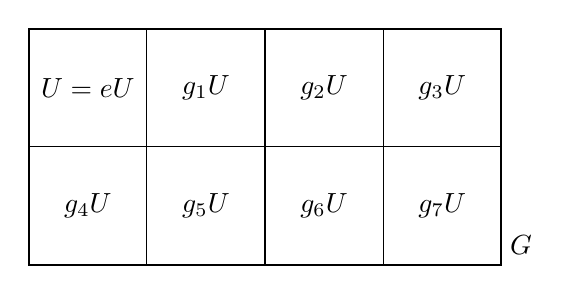
\begin{tikzpicture}
            \draw[thick] (0,0) rectangle (6, 3);
            \draw (0,1.5) -- (6,1.5) (1.5,0) -- (1.5,3) (3,0) -- (3,3) (4.5, 0) -- (4.5, 3);
            \node at (6.25, 0.25) {$G$};  
            \node at (0.75, 2.25) {$U = eU$};
            \node at (2.25, 2.25) {$g_1U$};
            \node at (3.75, 2.25) {$g_2U$};
            \node at (5.25, 2.25) {$g_3U$};
            \node at (0.75, 0.75) {$g_4U$};
            \node at (2.25, 0.75) {$g_5U$};
            \node at (3.75, 0.75) {$g_6U$};
            \node at (5.25, 0.75) {$g_7U$};
        \end{tikzpicture}
        \caption{Nebenklassenzerlegung einer endlichen Gruppe}
    \end{figure}
\end{remark}

\begin{remark}
    Es gilt auch für Gruppen mit unendlicher Trägermenge, dass es gleich viele Linksnebenklassen wie Rechtsnebenklassen gibt. Es kann dafür die Funktion $\varphi: gU \mapsto Ug^{-1}$ definiert werden und gezeigt werden, dass diese wohldefiniert und bijektiv ist.
\end{remark}

\begin{theorem}[Lagrange]\index{Satz!von Lagrange}
    Sei $G$ eine endliche Gruppe, $U \le G$ eine Untergruppe und $g \in G$. Dann gilt
    \begin{itemize}
        \item $\vert U \vert$ teilt $\vert G \vert$ und
        \item $\ord(g)$ teilt $\vert G \vert $.
    \end{itemize}
\end{theorem}
\begin{proof}
    Die erste Behauptung folgt aus \cref{rem:nebenklassenzerlegung_endlich}, für die zweite wählen wir $U := \langle g \rangle$.
\end{proof}

\begin{example}
    Betrachten wir $(\mathbb{Z}_6, +, 0, -)$ mit Ordnung 6. Es sind dann $\ord(0) = 1, \ord(1) = \ord(5) = 6, \ord(2) = \ord(4) = 3, \ord(3) = 2$, welche alle Teiler von 6 sind.

    Sei $G$ eine Gruppe mit $\vert G \vert = p \in \mathbb{P}$. Für $g \in G\setminus\{e\}$ gilt nun $\ord(g) = p \Rightarrow \langle g \rangle = G$, womit $G$ zyklisch ist. Gruppen mit Primzahlordnung sind also zyklisch.
\end{example}

\begin{definition}
    Sei $G$ eine Gruppe und $U \le G$ eine Untergruppe. Der \emph{Index von $U$ in $G$}\index{Index} ist definiert als $[G:U] := \vert \{gU \mid g \in G\}\vert = \vert \{Ug \mid g \in G\}\vert$. 
\end{definition}

\begin{remark}
    Ist $G$ endlich, dann haben wir in \cref{rem:nebenklassenzerlegung_endlich} $[G:U] = \frac{\vert G \vert}{\vert U \vert}$ gezeigt.
\end{remark}

\begin{theorem}[Indexsatz]\index{Indexsatz}
    Sei $G$ eine Gruppe und seien $V \le U \le G$ Untergruppen, dann ist $$[G:V] = [G:U] \cdot [U:V].$$ 
\end{theorem}
\begin{proof}
    Wurde in der Übung bewiesen.
\end{proof}

Im Allgemeinen ist die durch Links-/Rechtsnebengruppen induzierte Äquivalenzrelation keine Kongruenzrelation. Der folgende \cref{theorem:normalteiler_equiv} liefert Bedingungen, wann dies erfüllt ist.

\begin{definition}
    Sei $G$ eine Gruppe, dann heißt eine Teilmenge $N \subseteq G$ \emph{Normalteiler}\index{Normalteiler}, wenn eine der Bedingungen aus \cref{theorem:normalteiler_equiv} erfüllt ist. Man schreibt $N\vartriangleleft G$.
\end{definition}

\begin{theorem}\label{theorem:normalteiler_equiv}
    Sei $G$ eine Gruppe, $N \subseteq G$, dann sind äquivalent:
    \begin{enumerate}[label=(\enumArabicDual*)]
        \item\label{item:theorem:normalteiler_equiv_1} Es gibt genau eine Kongruenzrelation $\sim$ auf $G$ mit $N = [e]_\sim$, nämlich $x \sim y: \Leftrightarrow x^{-1}y \in N$.
        \item\label{item:theorem:normalteiler_equiv_1'} Es gibt eine Kongruenzrelation $\sim$ auf G mit $N = [e]_\sim$.
        \item\label{item:theorem:normalteiler_equiv_2} Es gibt eine Gruppe $H$ und einen surjektiven Homomorphismus $\varphi: G \to H$ mit $N = \varphi^{-1}(\{e_H\})$.
        \item\label{item:theorem:normalteiler_equiv_2'} Es gibt eine Gruppe $H$ und einen Homomorphismus $\varphi: G \to H$ mit $N = \varphi^{-1}(\{e_H\})$.
        \item\label{item:theorem:normalteiler_equiv_3} Es ist $N \le G$ mit $\forall x \in G: xNx^{-1} = N$.
        \item\label{item:theorem:normalteiler_equiv_3'} Es ist $N \le G$ mit $\forall x \in G: xNx^{-1} \subseteq N$.
        \item\label{item:theorem:normalteiler_equiv_4} Es ist $N \le G$ mit $\forall x \in G: xN = Nx$.
        \item\label{item:theorem:normalteiler_equiv_4'} Es ist $N \le G$ mit $\forall x \in G: xN \subseteq Nx$.
    \end{enumerate}
\end{theorem}


\begin{proof}{\ }
    \begin{itemize}[topsep=0cm, leftmargin=2.2cm]
        \item[\ref*{item:theorem:normalteiler_equiv_1} $\Rightarrow$ \ref*{item:theorem:normalteiler_equiv_1'}:] 
        Trivial.
        
        \item[\ref*{item:theorem:normalteiler_equiv_1'} $\Rightarrow$ \ref*{item:theorem:normalteiler_equiv_2}:] 
        Wählen wir $H = G/_\sim$ und sei $\varphi: G \to H, g \mapsto [g]_\sim$ die kanonische Einbettung. Es ist dann klarerweise $\varphi$ surjektiv und $\varphi^{-1}(\{e_H\}) = [e]_\sim = N$.
        
        \item[\ref*{item:theorem:normalteiler_equiv_2} $\Rightarrow$ \ref*{item:theorem:normalteiler_equiv_2'}:] 
        Trivial.
        
        \item[\ref*{item:theorem:normalteiler_equiv_2'} $\Rightarrow$ \ref*{item:theorem:normalteiler_equiv_3'}:] 
        Zeigen wir zuerst, dass $N$ eine Untergruppe ist. Seien dazu $n, n' \in N = \varphi^{-1}(\{e_H\})$. Dann ist $\varphi(n n') = \varphi(n) \varphi(n') = e_H e_H = e_H$, womit $n n' \in \varphi^{-1}(\{e_H\}) = N$ ist.
        Zuletzt ist für $n\in N$ auch $n^{-1}\in N$ nötig. Das gilt wegen $\varphi(n^{-1})=\varphi(n)^{-1}=e^{-1}=e$, daher ist $N \le G$.

        Zeigen wir nun noch für $x \in G, n \in N$, dass $y = xnx^{-1} \in N$ ist. Wir erhalten $$\varphi(y) = \varphi(x) \underbrace{\varphi(n)}_{= e_H} \varphi(x^{-1}) = \varphi(x)\varphi(x)^{-1} = e_H \;\Rightarrow\; y \in \varphi^{-1}(\{e_H\}) = N.$$

        \item[\ref*{item:theorem:normalteiler_equiv_3'} $\Rightarrow$ \ref*{item:theorem:normalteiler_equiv_3}:] 
        Wir wissen bereits, dass $\forall x \in G: xNx^{-1} \subseteq N$ gilt und wollen zeigen, dass für alle $y \in G$ die umgekehrte Inklusion gilt. Es ist $y^{-1} \in G$, womit $y^{-1}N(y^{-1})^{-1} = y^{-1}Ny \subseteq N$ ist. Wir erhalten damit nun 
        $$ N = (y y^{-1}) N (y y^{-1}) \overset{(*)}{=} y (y^{-1} N y) y^{-1} \subseteq y N y^{-1}, $$
        wobei $(*)$ einfach nachzurechnen ist.
        
        \item[\ref*{item:theorem:normalteiler_equiv_3} $\Rightarrow$ \ref*{item:theorem:normalteiler_equiv_4}:] 
        Zeigen wir für $x \in G$, dass $xN \subseteq Nx$ ist. Für ein $y \in xN$ gibt es ein $n \in N$, sodass $y = xn$. Wählen wir $n' = yx^{-1} = xnx^{-1} \in xNx^{-1} = N$, so ist $y = n'x$ und damit $y \in Nx$. Die andere Mengeninklusion zeigt man analog. 
        
        \item[\ref*{item:theorem:normalteiler_equiv_4} $\Rightarrow$ \ref*{item:theorem:normalteiler_equiv_4'}:] 
        Trivial.
        
        \item[\ref*{item:theorem:normalteiler_equiv_4'} $\Rightarrow$ \ref*{item:theorem:normalteiler_equiv_1}:]  
        Zeigen wir zuerst die Eindeutigkeit: Sei angenommen es gibt eine Kongruenzrelation $\sim$ auf $G$ mit $N = [e]_\sim$. Für $x, y\in G$ gilt dann 
        \begin{itemize}
            \item $x \sim y \;\Rightarrow\; x^{-1}x \sim x^{-1}y \; \Leftrightarrow\; e \sim x^{-1}y \;\Leftrightarrow\; x^{-1}y \in [e]_\sim = N$ und
            \item $x^{-1}y \in N = [e]_\sim \;\Leftrightarrow\; e \sim x^{-1}y \;\Leftrightarrow\; x = xe \sim x(x^{-1}y) = y$.
        \end{itemize}
        Es ist dann also $x \sim y \Leftrightarrow x^{-1}y \in N$. 
        
        Zeigen wir nun noch, dass dieses $\sim$ eine Kongruenzrelation auf $G$ ist. Nach \cref{lemma:euqivrel_linksnebenklassen} ist $\sim$ eine Äquivalenzrelation, bleibt also noch die Invarianz unter $G$ zu zeigen. 
        \begin{itemize}
            \item Zeigen wir für $x,x',y,y' \in G$ mit $x \sim y, x' \sim y'$, dass $xx'\sim yy'$. Es gilt 
            $$ xx'\sim yy' \;\Leftrightarrow\; x'^{-1}\underbrace{x^{-1}y}_{=: n \in N} y' = \underbrace{x'^{-1} n}_{\in x'^{-1}N \subseteq Nx'^{-1}} y' \overset{(*)}{=} n'\underbrace{x'^{-1}y'}_{\in N} \in N, $$
            wobei wir bei $(*)$ verwenden, dass nach \ref*{item:theorem:normalteiler_equiv_4'} ein $n' \in N$ existiert, sodass $x'{-1} n = n' x'{-1}$.
            \item Zeigen wir für $x,y \in G$ mit $x \sim y$, dass $x^{-1} \sim y^{-1}$. Es gilt
            $$ x\sim y \;\Leftrightarrow\; x^{-1}x \sim x^{-1}y \;\Leftrightarrow\; e \sim x^{-1}y \;\Leftrightarrow\; ey^{-1} \sim x^{-1} y y^{-1} \;\Leftrightarrow\; y^{-1} \sim x^{-1}.$$ 
            \item Klarerweise ist $e \sim e$, also ist $\sim$ invariant unter der 0-stelligen Operation $e$.
        \end{itemize}
    \end{itemize}
\end{proof}

\begin{remark}
    \cref{theorem:normalteiler_equiv} beschreibt einige Eigenschaften von Normalteilern.
    \begin{itemize}
        \item \ref*{item:theorem:normalteiler_equiv_1}, \ref*{item:theorem:normalteiler_equiv_1'} liefern den bijektiven Zusammenhang von Normalteilern und Kongruenzrelation. Betrachtet man die Verbände von Normalteilern bzw. Kongruenzrelationen, so stellt diese Bijektion einen Verbandsisomorphismus dar.
        \item \ref*{item:theorem:normalteiler_equiv_2}, \ref*{item:theorem:normalteiler_equiv_2'} beschreiben die Darstellung des Normalteilers über den Kern eines Homomorphismus $\varphi: G \to H$. Es ist $\ker \varphi = \{g \in G \mid \varphi(g) = e_H\} = \varphi^{-1}(\{e_H\}) = N$.
        \item \ref*{item:theorem:normalteiler_equiv_3}, \ref*{item:theorem:normalteiler_equiv_3'} liefern direkt, dass Normalteiler unter Abbildungen $\pi_x: G \to G, g \mapsto xgx^{-1}$ abgeschlossen sind. So eine Abbildung nennt man \emph{inneren Automorphismus}\index{innerer Automorphismus}.
        \item \ref*{item:theorem:normalteiler_equiv_4}, \ref*{item:theorem:normalteiler_equiv_4'} besagen, dass die Links- und Rechtsnebenklassen einer Untergruppe genau dann gleich sind, wenn die Untergruppe ein Normalteiler ist.
    \end{itemize}

    Inbesondere sind alle Äquivalenzklassen einer Kongruenzrelation gleich groß, da sie lediglich ``Verschiebungen'' der Äquivalenzklasse des neutralen Elements sind.
\end{remark}

\begin{corollary} \label{corollary:abelsch-normalteiler-untergruppe}
    In einer abelschen Gruppe $G$ ist $N \subseteq G$ genau dann ein Normalteiler, wenn $N$ eine Untergruppe von $G$ ist.
\end{corollary}
\begin{proof}
    In einer abelschen Gruppe ist immer $xN = Nx$. \cref{theorem:normalteiler_equiv} \ref*{item:theorem:normalteiler_equiv_4} liefert dann damit die Behauptung.
\end{proof}

\notedate{19.04.2023}

\begin{remark} \label{remark:gruppe-injektiv-kern-trivial}
    Seien $G, H$ Gruppen, $h : G \to H$ ein Homomorphismus. Es sei erinnert, dass $h$ injektiv ist, wenn
    $$ \{ (x,y) \mid h(x) = h(y) \} = \{ (x,x) \mid x \in G \}. $$
    Erstere Menge definiert eine Kongruenzrelation $\sim$ auf $G$. Also ist $h$ genau dann injektiv, wenn $\sim$ die triviale Gleichheitsrelation ist, also $[e]_\sim = \{e\}$, also gerade $\ker h = \{ e \}$. Man vergleiche diese Eigenschaft mit der Injektivität von Vektorraum-Homomorphismen aus der Linearen Algebra.
\end{remark}

\begin{remark}
    Es sei an \cref{def:einfache-algebra} einer einfachen Algebra erinnert. Wir bemerken, dass eine Gruppe genau dann einfach ist, wenn sie nur ihre Trägermenge und $\{e\}$ als Normalteiler hat.
\end{remark}

\begin{definition}
    Sei $G$ eine Gruppe, $N \vartriangleleft G$ ein Normalteiler und $\sim$ die entsprechende Kongruenzrelation. Wir definieren die \emph{Faktorgruppe} \index{Gruppe!Faktor-}
    $$ G /_N := G /_\sim = \{ aN \mid a \in G \}. $$
    Dabei ist
    $$ aN \cdot bN := (a \cdot b)N. $$
    Man überzeugt sich leicht davon, dass dies gerade dann wohldefiniert ist wenn eben $N$ ein Normalteiler ist.
\end{definition}

\begin{example}
    Betrachte die Gruppe $(\mathbb{Z}, +, 0, -)$, so ist für jedes $m \in \mathbb{N}$ die Menge $m \mathbb{Z}$ eine Untergruppe, und da sie kommutativ ist nach \cref{corollary:abelsch-normalteiler-untergruppe} auch ein Normalteiler.

    Sei $\sim$ die entsprechende Kongruenzrelation und betrachten wir $(\mathbb{Z}, +, 0, -)/_\sim$, so enthält diese Faktorgruppe
    $$ 0 + m\mathbb{Z}, \quad 1 + m\mathbb{Z}, \quad \hdots, \quad (m-1) + m\mathbb{Z}. $$

    In dieser Gruppe rechnet man
    $$ (i + m\mathbb{Z}) + (j + m\mathbb{Z}) = (i+j) + m\mathbb{Z}, $$
    wobei man auch $(i + j \pmod{m})$ für einen ``schöneren'' Repräsentanten betrachten kann.

    Im Falle $n = 4$ ist beispielsweise
    $$ (1 + 4\mathbb{Z}) + (3 + 4\mathbb{Z}) = 4 + 4\mathbb{Z} = 0 + 4\mathbb{Z}. $$
\end{example}

\begin{example}
    Betrachte die Gruppe $(\Gl_2(\mathbb{R}), \cdot, E_2, {}^{-1})$ und
    $$ N := \{ A \in \Gl_2(\mathbb{R}) \mid \det A = 1 \}. $$
    Für ein beliebiges $A \in \Gl_2(\mathbb{R})$ gilt $ A N A^{-1} \subseteq N, $ da mit $C \in N$
    $$ \det(A C A^{-1}) = \det A \det C \det A^{-1} = \det C = 1. $$
    Also ist $N$ ein Normalteiler. Sei $\sim$ die entsprechende Äquivalenzrelation, wir wollen die Struktur von $\Gl_2(\mathbb{R})/_\sim$ analysieren. Es gilt
    $$ A \sim B \Leftrightarrow A \cdot B^{-1} \in N \Leftrightarrow \det(A \cdot B^{-1}) = 1 \Leftrightarrow \det A = \det B, $$
    die Äquivalenzklassen hängen also nur von der Determinante und ansonsten nicht von der unterliegenden Matrixstruktur ab. Also ist $\Gl_2(\mathbb{R})/_\sim \cong (\mathbb{R} \setminus \{0\}, \cdot, 1, {}^{-1})$.
\end{example}

\begin{remark}
    Sei $G$ eine Gruppe, $\sim$ eine Kongruenzrelation und $N=[e]_\sim$. Wir fragen uns, wann $G/_\sim$ kommutativ ist. Dazu bemerken wir
    $$ G/_\sim \textrm{ kommutativ} \quad \Leftrightarrow \quad \forall a, b \in G: (ab)N = (aN) (bN) = (bN) (aN) = (ba)N. $$
    Letzteres können wir umschreiben als $a^{-1} b^{-1} a b N = N$, was genau dann der Fall ist, wenn für beliebiges $a, b$ gilt
    $$ [a, b] := a^{-1} b^{-1} a b \in N. $$
    Wir nennen $[a, b]$ den \emph{Kommutator} \index{Kommutator} von $(a, b)$.
\end{remark}

\begin{definition}
    Definiere
    $$ G' := \langle \{ [a, b] \mid a, b \in G \} \rangle \leq G. $$
    Wir nennen $G'$ die \emph{Ableitung} oder auch die \emph{Kommutatorgruppe} von $G$. \index{Gruppe!Ableitung}\index{Gruppe!Kommutatorgruppe}
\end{definition}
    
\begin{proposition}
    Sei $G$ eine Gruppe. Ist $G$ abelsch, so ist $G' = \{ e \}$.
\end{proposition}

\begin{proof}
    Ist $G$ abelsch so ist
    $$ G' = \langle \{ a^{-1} b^{-1} a b \mid a, b \in G \} \rangle = \langle \{ a^{-1} b^{-1} b a \mid a, b \in G \} \rangle = \langle \{e\} \rangle = \{e\}. $$
\end{proof}

\begin{theorem}
    Sei $G$ eine Gruppe. Dann gilt:
    \begin{enumerate}
        \item $G' \vartriangleleft G$
        \item $G/_{G'}$ ist abelsch.
        \item $\forall N \vartriangleleft G: ( G/_N \textrm{ abelsch} \Leftrightarrow N \supseteq G')$
    \end{enumerate}
\end{theorem}

\begin{proof}
    (2) ist ein Spezialfall von (3).

    Um (3) einzusehen sei $N \vartriangleleft G$, so folgt mit obiger Bemerkung sofort
    \begin{align*}
        G/_N \textrm{ abelsch} &\Leftrightarrow \forall a, b: (aN)(bN) = (bN)(aN) \Leftrightarrow \\ &\Leftrightarrow \forall a, b: a^{-1}b^{-1} a b \in N \Leftrightarrow \forall a, b: [a, b] \in N \Leftrightarrow N \supseteq G'.
    \end{align*}

    Zeigen wir nun (1). Sei $h : G \to G$ ein beliebiger Endomorphismus, dann gilt für alle $a, b \in G$, dass $h([a,b]) = [h(a), h(b)]$, also $h(G') \subseteq G'$. Für beliebiges $x \in G$ definieren wir
    $$ h_x : G \to G, g \mapsto xgx^{-1}, $$
    so ist $h_x$ ein Automorphismus\footnote{$h_x$ ist wie früher schon bemerkt ein \emph{innerer Automorphismus}.}. Also ist
    $$ x G' x^{-1} = h_x(G') \subseteq G', $$
    womit $G' \vartriangleleft G$ folgt.
\end{proof}

\subsection{Innere direkte Produkte}

\begin{definition}
    Sei $G$ eine Gruppe, $U_1, U_2 \subseteq G$, so definieren wir das \emph{Komplexprodukt}\index{Komplexprodukt}
    $$ U_1 \cdot U_2 = \{ u_1 \cdot u_2 \mid u_1 \in U_1, u_2 \in U_2 \}. $$
\end{definition}

\begin{definition} \label{def:direktes-inneres-produkt}
    Sei $G$ eine Gruppe, $U_1, \hdots, U_n \leq G$. Wir nennen $G$ ein \emph{inneres direktes Produkt}\index{inneres direktes Produkt} von $(U_1, \hdots, U_n)$, wenn die Abbildung
    $$ \varphi : U_1 \times \hdots \times U_n \to G, (u_1, \hdots u_n) \mapsto u_1 \cdot \hdots \cdot u_n $$
    ein Isomorphismus ist. In diesem Fall schreiben wir $G = U_1 \odot \hdots \odot U_n$.
\end{definition}

\begin{remark} \label{remark:inneres-direktes-produkt-notwendig}
    Wir sammeln nun notwendige Bedingungen dafür, dass $G$ ein inneres direktes Produkt ist.
    
    Für $i \in \{ 1,\hdots,n \}$ definiere $V_i := U_1 \cdot \hdots \cdot U_{i-1} \cdot U_{i+1} \cdot \hdots \cdot U_n$, so muss gelten
    $$ U_i \cap V_i = \{ e \}. $$
    Sonst gäbe es $(u_j)_{j=1}^n \in (U_j)_{j=1}^n, u_i \neq e$ mit
    $$ \varphi(e, \hdots, e, \overbrace{u_i}^{\textrm{$i$-te Stelle}}, e, \hdots, e) = u_i \overset{!}{=} u_1 \cdot \hdots \cdot u_{i-1} \cdot u_{i+1} \cdot \hdots \cdot u_n = \varphi(u_1, \hdots, u_{i-1}, e, u_{i+1}, \hdots, u_n), $$
    womit $\varphi$ nicht injektiv wäre.

    Weiters muss $U_i \vartriangleleft G$ sein. Um dies einzusehen, betrachte die Abbildung
    $$ \psi_i : U_1 \times ... \times U_n \to U_1 \times ... \times U_{i-1} \times U_{i+1} \times ... \times U_n, (u_i)_{i=1}^n \mapsto (u_i, \hdots, u_{i-1}, u_{i+1}, \hdots, u_n). $$
    Diese ist ein Homomorphismus, womit
    $$ \ker \psi_i = \{e\} \times ... \times \{e\} \times U_i \times \{e\} \times ... \times \{e\} \vartriangleleft U_1 \times ... \times U_n. $$
    Damit ist $U_i = \varphi(\ker \psi_i) \vartriangleleft G$.

    Zuletzt gilt in einem direkten inneren Produkt für $i \neq j, x \in U_i, y \in U_j$, dass $xy = yx$. Um dies einzusehen sei \obda $i < j$, so gilt
    \begin{align*}        
        xy &= \varphi(e, \hdots, e, \overbrace{x}^{\textrm{$i$-te Stelle}}, e, \hdots, e) \cdot \varphi(e, \hdots, e, \overbrace{y}^{\textrm{$j$-te Stelle}}, e, \hdots, e) =  \\ &= \varphi(e, \hdots, e, \overbrace{x}^{\textrm{$i$-te Stelle}}, e, \hdots, e, \overbrace{y}^{\textrm{$j$-te Stelle}}, e, \hdots, e) = \\ &= \varphi(e, \hdots, e, \overbrace{y}^{\textrm{$i$-te Stelle}}, e, \hdots, e) \cdot \varphi(e, \hdots, e, \overbrace{x}^{\textrm{$j$-te Stelle}}, e, \hdots, e) = yx.
    \end{align*}
\end{remark}

\begin{lemma} \label{lemma:gruppe-normalteiler-kommutativ}
    Sei $G$ eine Gruppe, $U, V \vartriangleleft G$, $U \cap V = \{ e \}$, dann gilt für alle $u \in U$ und $v \in V$, dass $uv = vu$.
\end{lemma}

\begin{proof}
    Es gilt
    $$ uv = vu \Leftrightarrow u^{-1} v^{-1} u v = e. $$
    Nun ist $u^{-1} v^{-1} u \in V$, damit $u^{-1} v^{-1} u v \in V$. Andererseits gilt $v^{-1} u v \in U$, damit $u^{-1} v^{-1} u v \in U$. Also folgt $u^{-1} v^{-1} u v = e$ und damit $uv=vu$.
\end{proof}

\begin{proposition} \label{prop:kriterien-direktes-inneres-produkt}
    Sei $G$ eine Gruppe und $U_1, \hdots, U_n \leq G$. Gelte $G = U_1 \cdot \hdots \cdot U_n$, beziehungsweise äquivalent die Surjektivität von $\varphi$ wie in \cref{def:direktes-inneres-produkt}. Gelte weiters für $i \in \{ 1, \hdots, n \} $, dass $U_i \vartriangleleft G$ und $U_i \cap V_i = \{ e \} $, wobei $V_i$ wie in \cref{remark:inneres-direktes-produkt-notwendig} definiert ist. Dann ist $G = U_1 \odot \hdots \odot U_n $.
\end{proposition}

\begin{proof}
    Zeigen wir, dass $\varphi$ ein Homomorphismus ist. Mit \cref{lemma:gruppe-normalteiler-kommutativ} gilt
    \begin{align*}        
        \varphi((u_1, \hdots, u_n) \cdot (v_1, \hdots, v_n)) &= \varphi(u_1 v_1, \hdots, u_n v_n) = u_1 v_1 \hdots u_n v_n = \\ &= u_1 \hdots u_n v_1 \hdots v_n = \varphi(u_1, \hdots, u_n) \varphi(v_1, \hdots, v_n).
    \end{align*}

    Bleibt die Injektivität zu zeigen. Dazu reicht es nach \cref{remark:gruppe-injektiv-kern-trivial} zu zeigen, dass der Kern trivial ist. Sei also $\varphi(u_1, \hdots, u_n) = e$, so ist $(u_1, \hdots, u_n) = (e, \hdots, e)$ zu zeigen. Sei dazu indirekt angenommen es wäre nicht der Fall und sei $i$ minimal mit $u_i \neq e$, also
    $$ e = \varphi(u_1, \hdots, u_n) = e \hdots e u_i \hdots u_n = u_i \hdots u_n, $$
    womit $u_i^{-1} = u_{i+1} ... u_n \in V_i$ folgt. Da jedoch auch $u_i^{-1} \in U_i$ und $U_i \cap V_i = \{ e \}$ folgt damit $u_i = e$, im Widerspruch.

    Insgesamt ist $\varphi$ also ein Isomorphismus, was zu zeigen war.
\end{proof}

\begin{remark}
    Sei $(U_i)_{i \in I}$ eine Familie von Untergruppen einer Gruppe $G$, wobei $(I, <)$ totalgeordnet ist. Wir definieren das \emph{schwache Produkt} \index{schwaches Produkt}
    $$ \prod_{i \in I}^w U_i := \{ f : I \to \bigcup_{i \in I} U_i \mid \forall i \in I: f(i) \in U_i \land f(i) = e \textrm{ für fast alle } i \in I \}. $$
    Definiere weiters
    $$ \varphi : \prod_{i \in I}^w U_i \to G, f \mapsto f(i_1) \cdot \hdots \cdot f(i_k), $$
    wobei $i_1 < \hdots < i_k $ genau jene Indizes sind, für die $f(i_j) \neq e$ ist.

    Falls $\varphi$ ein Isomorphismus ist, so nennen wir $G$ \emph{inneres direktes Produkt} von $(U_i)_{i \in I}$.

    Ohne Beweis sei angemerkt dass \cref{prop:kriterien-direktes-inneres-produkt} entsprechend auch für solche inneren direkten Produkte gilt.
\end{remark}

\notedate{20.04.2023}

\subsection{Zyklische Gruppen}

Es sei an die Definition einer zyklischen Gruppe in \cref{def:gruppe} erinnert.

\begin{example}
    $\mathbb{Z} = \langle \{1\}\rangle$ und $\mathbb{Z}_m = \langle\{1\}\rangle$ sind zyklische Gruppen.
\end{example}

\begin{proposition}\label{prop:zyklische_gruppen_1} Für eine Gruppe $G$ gilt:
    \begin{enumerate}
        \item $G\;\text{zyklisch} \Leftrightarrow \exists h: \mathbb{Z} \to G\;\text{surjektiver Homomorphismus}$
        \item $G\;\text{zyklisch} \Rightarrow G\;\text{abelsch}$
        \item $G\;\text{zyklisch} \Rightarrow \forall F \in \textrm{H}(\{G\}): F\;\text{zyklisch}$
        \item $G\;\text{zyklisch} \Rightarrow \forall F \in \textrm{S}(\{G\}): F\;\text{zyklisch}$
    \end{enumerate}
\end{proposition}

\begin{proof} {\ }
    \begin{enumerate}
        \item \begin{itemize}
            \item[$\Leftarrow$:] Es gilt $\mathbb{Z}=\langle \{1\} \rangle$ und damit folgt $G=\langle \{h(1)\} \rangle$.
            \item[$\Rightarrow$:] Sei $g \in G$ so, dass $G = \{g^n \mid g \in \mathbb{Z}\} $. Definiere die Abbildung $h: \mathbb{Z} \to G, n \mapsto g^n$. Dafür gilt $h(0) = e_g$, $h(n)^{-1} = (g^{n})^{-1} = g^{-n} = h(-n)$ und $h(m+n) = g^{m+n} = g^m g^n = h(m)h(n)$, womit $h$ ein Homomorphismus ist. Aufgrund der Wahl von $g$ ist $h$ nun surjektiv.
        \end{itemize}
        \item Diese Aussage folgt direkt aus 1., da abelsche Gruppen eine Varietät bilden. Es ist $\mathbb{Z}$ abelsch, also auch dessen homomorphe Bilder, insbesondere $G$.
        \item Sei $F \in \mathrm{H}(\{G\})$ beliebig, es gibt also einen surjektiven Homomorphismus $\varphi: G \to F$. Aus 1. erhalten wir außerdem, da $G$ zyklisch ist, die Existenz eines surjektiven Homomorphismus $h: \mathbb{Z} \to G$. Die Verkettung $\varphi \circ h: \mathbb{Z} \to F$ ist nun erneut ein surjektiver Homomorphismus, weshalb wir erneut aus 1. erhalten, dass $F$ zyklisch ist.
        \item Sei $F \in \mathrm{S}(\{G\})$ beliebig, also $F \le G$. Weiter sei $h: \mathbb{Z} \to G$ ein nach 1. existierender surjektiver Homomorphismus.
        Wir wählen nun $U := h^{-1}(F) \le \mathbb{Z}$ und $m := \min\{n > 0 \mid n \in U\}$ bzw. $0$, falls die Menge leer ist. 
        
        Wir behaupten nun, dass $U = m \mathbb{Z}$. Sei zuerst $mk \in m\mathbb{Z}$, dann folgt, da $m \in U$ und $U$ als Untergruppe unter Addition und Inversenbildung abgeschlossen ist, induktiv auch $mk \in U$. Es gilt also $U \supseteq m\mathbb{Z}$. Sei nun $n \in U$ und \obda $n > 0$. Es gibt dann $k \in \mathbb{N}$ und $r \in \{0, \ldots, m-1\}$, sodass $n = mk+r$. Durch Umformen erhalten wir $r = n - mk \in U$. Aufgrund der Wahl von $m$ folgt nun, dass $r = 0$, da es sonst ein kleineres positives Element als $m$ in $G$ gäbe, im Widerspruch zur Minimalität von $m$. Es ist also $n = mk \in m\mathbb{Z}$, womit $U = m\mathbb{Z}$ folgt.

        Betrachten wir nun den surjektiven Homomorphismus $h\vert_{m\mathbb{Z}}: m\mathbb{Z} \to F$. Da $m\mathbb{Z} = \langle\{m\}\rangle$ und $m\mathbb{Z}$ damit zyklisch ist, folgt aus 1., dass $F$ zyklisch ist.
    \end{enumerate}
\end{proof}

\begin{remark}
    Es ist leicht einzusehen, dass $\mathbb{Z}_2 \times \mathbb{Z}_2$ nicht zyklisch ist, obwohl $\mathbb{Z}_2$ es ist. Die zyklischen Gruppen sind also nicht unter P abgeschlossen und daher keine Varietät.
\end{remark}

\begin{proposition}
    Sei $G$ eine zyklische Gruppe. Dann ist $G \cong \mathbb{Z}$ oder $G \cong \mathbb{Z}_m$.
\end{proposition}
\begin{proof}
    Aus \cref{prop:zyklische_gruppen_1} folgt die Existenz eines surjektiven Homomorphismus $h: \mathbb{Z} \to G$. Der Homomorphiesatz (\ref{satz:homomorphiesatz}) liefert, dass $G \cong \mathbb{Z}/_{\ker h}$. Ist $\ker h = \{0\}$, so ist $G \cong \mathbb{Z}$. Ist $\ker h$ nicht trivial, so gibt es ein $m \in \mathbb{N}$, sodass $\ker h = m\mathbb{Z}$, da der Kern immer eine Untergruppe ist und im Beweis von \cref{prop:zyklische_gruppen_1} gezeigt wurde, dass alle Untergruppen von $\mathbb{Z}$ diese Form haben. Es folgt also $G \cong \mathbb{Z}/_{m\mathbb{Z}} \cong \mathbb{Z}_m$.
\end{proof}

\begin{definition}
    Für $m\in\mathbb{N}\setminus\{0\}$ bezeichne mit $C_m$\footnote{Man verifiziert sofort, dass $C_m\cong\mathbb{Z}_m$ gilt, vermöge dem Isomorphismus $\varphi:C_m\to\mathbb{Z}_m,x\mapsto\{x+km\mid k\in\mathbb{Z}\}$.} die Gruppe $(\{0,\ldots,m-1\},+,0,-)$ wobei
    $$a+b:=\min\{n\geq 0\mid a+b\equiv n \;\mathrm{mod}(m)\}.$$
\end{definition}

\subsection{Symmetrische und Permutationsgruppen}

\begin{definition}
    Für eine Menge $A$ sei
    $$ S_A = \{f: A \to A \mid f \;\text{bijektiv}\}$$
    definiert. Wir nennen $(S_A, \circ, \id_A, {}^{-1})$ die \emph{symmetrische Gruppe von A}\index{Gruppe!symmetrische}.

    Jede Untergruppe $U \le S_A$ einer symmetrischen Gruppe heißt \emph{Permutationsgruppe}\index{Permutationsgruppe}.
\end{definition}

\begin{theorem}[Darstellungssatz von Cayley für Gruppen]\index{Satz!von Cayley (Gruppen)}\label{satz:darstellungssatz-cayley-gruppen}
    Sei $G$ eine Gruppe, dann existiert eine Permutationsgruppe $U$, sodass $G \cong U$.
\end{theorem}
\begin{proof}
    Definieren wir die Abbildungen $$f_g: G \to G, h \mapsto gh \quad\text{und}\quad \varphi: G \to G^G, g \mapsto f_g.$$
    Im Beweis von \cref{theorem:darstellungssatz-cayley-monoid} wurde bereits gezeigt, dass $\varphi$ ein injektiver Monoid-Homomorphismus bezüglich $\cdot / \circ$ ist. Sei nun $g \in G$ beliebig, dann gilt $$ \id_G = f_e = \varphi(e) = \varphi(g g^{-1}) = \varphi(g) \circ \varphi(g^{-1}) = f_g \circ f_{g^{-1}}$$
    und analog $f_{g^{-1}} \circ f_g = \id_G$, also sind diese invers zueinander und somit Bijektionen. Wir erhalten daraus nun, dass $\varphi(g)^{-1} = \varphi(g^{-1})$ gilt, also $\varphi$ ein Gruppenhomomorphismus ist und, dass $\varphi(G) \le S_G$.
\end{proof}

\begin{definition}
    Sei $A$ eine Menge und $G$ eine Gruppe. Ein Homomorphismus $h: G \to S_A$ heißt \emph{(Gruppen)Aktion von G auf A}\index{Gruppe!-aktion}. Man schreibt auch $G \overset{h}{\curvearrowright} A$.
\end{definition}

\begin{remark}
   Ein Beispiel einer Gruppenaktionen von $G$ nach $G$ ist also die Linkstranslation $\varphi$ aus dem Beweis von \cref{satz:darstellungssatz-cayley-gruppen}. Eine weitere bekannte Gruppenaktion ist die Abbildung
   \begin{equation*}
        \Psi: G \to G^G, g \mapsto [\psi_g: G \to G, h \mapsto ghg^{-1}]. \tag*{(Konjugation)}
   \end{equation*}

   Ist $G$ abelsch, so ist $\Psi(G) = \{\id_G\}$. Außerdem ist 
   $$ \ker \Psi = \{g \in G \mid \psi_g = \id_G\} = \{g \in G \mid \forall h \in G: ghg^{-1} = h\} = \{g \in G \mid \forall h \in G: gh = hg\}. $$
\end{remark}

\begin{definition}
    Sei $G$ eine Gruppe. Dann ist das \emph{Zentrum von $G$}\index{Gruppe!Zentrum} definiert als
   $$ Z(G) := \{ g \in G \mid \forall h \in G: gh = hg\}. $$ 
\end{definition}

\begin{definition}
    Eine \emph{Permutation}\index{Permutation} ist eine bijektive Abbildung $\pi: \{1, \ldots, n\} \to \{1, \ldots, n\}$. Eine Darstellung von Permutationen ist die sogenannte \emph{Zyklenschreibweise}\index{Zyklenschreibweise}. Es wird die Permutation dabei dargestellt als
    $$ (a_1\; \pi(a_1)\; \pi^2(a_1)\; \ldots \; \pi^{\ell_{a_1} - 1}(a_1)) (a_2\; \pi(a_2)\; \ldots \; \pi^{\ell_{a_2} - 1}(a_2)) \ldots (a_n\; \pi(a_n)\; \ldots \; \pi^{\ell_{a_n} - 1}(a_n)),$$
    wobei die einzelnen Klammern \emph{Zyklus (von $a_i$)} genannt werden und $\ell_{a_i}$ die kleinste natürliche Zahl ist, sodass $\pi^{\ell_{a_i}}(a_i) = a_i$ gilt. Zyklen mit $\ell_{a_i} = 1$ (Fixpunkte) können in der Zyklenschreibweise weggelassen werden.
    Die Gruppe aller Permutationen für bestimmtes $n \in \mathbb{N}$ ist die \emph{symmetrische Gruppe}\index{symmetrische Gruppe} und wir schreiben auch $S_n := S_{\{1,\ldots, n\}}$.

    Eine \emph{Transposition}\index{Transposition} ist eine Permutation der Form $(i\; j)$.
\end{definition}

\begin{proposition}\label{prop:sym_gruppe} Für $n \in \mathbb{N}_{\ge 2}$ gilt
    \begin{enumerate}
        \item $\vert S_n \vert = n!$,
        \item $\forall \pi \in S_n: \pi\;\text{ist das Produkt von Transpositionen}$ und
        \item $\forall \pi \in S_n: \text{\# der Transpositionen modulo 2 ist unabhängig von der Darstellung}$.
    \end{enumerate}
\end{proposition}
\begin{proof}{\ }
    \begin{enumerate}
        \item Wir beweisen mittels vollständiger Induktion, dass es $n!$ Bijektionen zwischen zwei $n$-elementigen Mengen $X_n = \{x_1, \ldots, x_n\}, Y_n = \{y_1, \ldots, y_n\}$ gibt.
        
        Induktionsanfang ($n = 1$): Es gibt genau eine (bijektive) Abbildung $f: \{x_1\} \to \{y_1\}$.\\
        Induktionsschritt ($n \to n+1$): Für $i \in \{1, \ldots, n+1\}$ gibt es wegen der Induktionsvoraussetzung genau $n!$ Bijektionen von $X_n$ nach $\{y_1, \ldots, y_{i-1}, y_{i+1}, \ldots, y_{n+1}\}$, also gibt es $n!$ Bijektionen zwischen $X_{n+1}$ und $Y_{n+1}$ mit $f(x_{n+1}) = y_i$. Da nun $i$ aus $n+1$ Zahlen gewählt werden kann, gibt es $(n+1)n! = (n+1)!$ Bijektionen zwischen $X_{n+1}$ und $Y_{n+1}$.

        Mit $X_n = Y_n = \{1, \ldots, n\}$ folgt die Behauptung.

        \item Wir zeigen die Aussage mittels vollständiger Induktion:
        
        Induktionsanfang ($n = 2$): Es ist $S_n = \{ \id_{\{1,2\}}, (1\; 2) \}$, wobei $\id_{\{1,2\}} = (1\; 2) \circ (1\; 2)$.\\
        Induktionsschritt ($n \to n+1$): Sei $\pi \in S_{n+1}$. Falls $\pi(n+1) \not= n+1$ wählen wir die (selbstinverse) Transposition $\tau = (\pi(n+1)\; n+1)$. Wählen wir nun $\tilde{\pi} := \tau \circ \pi$ oder $\tilde{\pi} = \pi$ falls $\pi(n+1) = n+1$. Es ist dann $\tilde{\pi}\vert_{\{1,\ldots,n\}} \in S_n$, womit es nach der Induktionsvoraussetzung eine Darstellung als Produkt von Transpositionen gibt. Da $\pi = \tilde\pi$ oder $\pi = \tau\tilde\pi$ gibt es nun also auch für $\pi$ eine solche Darstellung.

        \item Sei $\pi \in S_n$ mit zwei Darstellungen $\pi = (i_1\; j_1) \hdots (i_k\; j_k) = (a_1\; b_1) \hdots (a_\ell\; b_\ell)$. Transposition sind selbstinvers, wir haben also
        $$ (a\ell\; b_\ell) \hdots (a_1\; b_1) (i_1\; j_1) \hdots (i_k\; j_k) = \id_{\{1,\hdots,n\}}. $$
        Es reicht also zu zeigen, dass die Identität keine ungerade Darstellung besitzt. Dazu bemerken wir, dass $S_n$ auf der Menge $M := \{ (i, j) \mid 1 \leq i, j \leq n, i \neq j \}$ als Gruppenaktion agiert, und zwar durch
        $$ \pi((i, j)) := (\pi(i), \pi(j)). $$
        Sei $(i, j) \in M, i < j$, dann nennen wir $(i,j)$ einen Fehlstand von $\pi$, wenn $\pi(i) > \pi(j)$. Sei $1 \leq a < b \leq n$ und betrachte die Transposition $\pi_{ab}$ von $a$ und $b$. Ein Fehlstand muss klarerweise immer $a$ oder $b$ enthalten. Dann hat $\pi_{ab}$ die Fehlstände $(a, b)$, $(a, j)$, wobei $a < j < b$ und $(j, b)$, wobei $a < j < b$. Insgesamt ist die Anzahl der Fehlstände also ungerade. Da eine ungerade Anzahl an Kompositionen an Transpositionen immer eine ungerade Anzahl an Fehlständen hat, die Identität jedoch eine gerade Anzahl hat (nämlich 0), kann die Identität also nicht aus einer ungeraden Anzahl von Permutationen erzeugt werden.
    \end{enumerate}
\end{proof}

\begin{corollary}
    Die Abbildung $$\sgn: S_n \to \{-1,1\}, \pi \mapsto \text{\# Transpositionen in der Darstellung von}\;\pi\;\text{mod}\; 2$$ ist ein Gruppenhomomorphismus.
\end{corollary}
\begin{proof}
    Zuerst bemerken wir, dass die Abbildung aufgrund von \cref{prop:sym_gruppe} wohldefiniert ist. Zeigen wir nun die Verträglichkeit mit den Operationen. Es gilt klarerweise $\sgn(\id) = 1$. Seien nun $\pi, \pi' \in S_n$. Betrachten wir den Fall, dass $\pi$ und $\pi'$ Darstellungen durch eine gerade Anzahl an Permutationen haben, dann hat auch $\pi \circ \pi'$ eine Darstellung durch eine gerade Anzahl an Permutationen und es gilt $\sgn(\pi)\sgn(\pi') = \sgn(\pi \circ \pi')$. Die anderen drei Fälle sind analog. Zuletzt sei noch $\pi \in G$, dann ist $1 = \sgn(\id) = \sgn(\pi \circ \pi^{-1}) = \sgn(\pi) \sgn(\pi^{-1})$. Ist nun $\sgn(\pi) = 1$, so folgt $\sgn(\pi^{-1}) = 1 = \sgn(\pi)^{-1}$, der andere Fall ist analog.
\end{proof}

\begin{remark}
    Es ist die \emph{alternierende Gruppe}\index{alternierende Gruppe} $A_n := \ker \sgn \vartriangleleft S_n$ ein Normalteiler der symmetrischen Gruppe. Mit dem Homomorphiesatz erhält man, dass $S_n/A_n \cong \ran \sgn = (\{-1,1\}, \cdot)$.
\end{remark}

\notedate{26.04.2023}

\subsection{Abelsche Gruppen}

\begin{remark}
    Sei $(G, \cdot, e, {}^{-1})$ eine abelsche Gruppe, so ist $G$ auch ein unitärer Modul über dem kommutativen 1-Ring $(\mathbb{Z}, +, 0, -, \ast, 1)$. Für $n \in \mathbb{Z}, g \in G$ definieren wir dazu $n \odot g := g^n$. Prüfen wir die Anforderungen an ein Modul. Seien $n, m \in \mathbb{Z}, g, h \in G$ beliebig. Dann ist
    $$ (n \ast m) \odot g = g^{n \ast m} = (g^m)^n = n \odot (m \odot g), $$
    $$ (n+m) \odot g = g^{n+m} = g^n \cdot g^m = (n \odot g) \cdot (m \odot g), $$
    $$ n \odot (g \cdot h) = (g \cdot h)^n = g^n \cdot h^n = (n \odot g) \cdot (n \odot h), $$
    $$1\odot g=g^1=g$$
    wobei wir bei der vorletzten Zeile verwenden, dass $G$ abelsch ist.

    Es stellt sich die Frage ob $G$ auch ein Modul über einem anderen Ring ist. Sei angenommen es gäbe ein $m \in \mathbb{Z}$, sodass für alle $g \in G$ gilt $g^m = e$. Dann ist $G$ ein unitärer Modul über $(\mathbb{Z}_m, +, 0, -, \ast, 1)$. Indirekt angenommen es gäbe ein $g \in G$ mit $g^m \neq e$, so wäre $g^0 = e$ ein Widerspruch.

    Im Folgenden wollen wir statt $\cdot, \ast, \odot$ stets nur $\cdot$ schreiben.
\end{remark}

\begin{definition}
    Der \emph{Exponent}\index{Gruppe!Exponent} einer Gruppe $G$ ist definiert als
    $$ \exp(G) := \min \{ m \in \mathbb{N} \setminus \{0\} \mid \forall g \in G: g^m = e \}, $$
    wobei wir $\exp(G) = \infty$ setzen, falls die obige Menge leer ist.
\end{definition}

\begin{remark}
    Ist $G$ also eine abelsche Gruppe mit $\exp(G) = m < \infty$, so ist $G$ ein unitärer $\mathbb{Z}_m$-Modul vermöge $k \odot g := g^k$ für $k \in \mathbb{Z}_m$.
\end{remark}

\begin{definition}
    Sei $G$ eine Gruppe, $g \in G, p \in \mathbb{P}$, so nennen wir $g$ ein \emph{$p$-Element}\index{Gruppe!$p$-Element}, wenn es ein $k \in \mathbb{N}$ mit $\ord(g) = p^k$ gibt. Weiters definieren wir den \emph{$p$-Anteil}\index{Gruppe!$p$-Anteil} von $G$ als
    $$ G_p := \{ g \in G \mid g \textrm{ ist $p$-Element } \}. $$
    Hier sei daran erinnert, dass $g$ \emph{Torsionselement}\index{Gruppe!Torsionselement} heißt, wenn es ein $k \in \mathbb{Z} \setminus \{ 0 \}$ mit $g^k = e$ gibt. Wir definieren die \emph{Torsionsgruppe von $G$}\index{Gruppe!Torsionsgruppe}:
    $$ G_t := \{ g \in G \mid g \textrm{ ist Torsionselement } \}. $$
\end{definition}

\begin{lemma} \label{lemma:abelsch-torsion-lemma}
    Sei $G$ eine abelsche Gruppe und seien $a_1, \hdots, a_n \in G_t$, so gelten:
    \begin{enumerate}
        \item $ \ord(a_1 \cdot \hdots \cdot a_n) \mid \ord(a_1) \cdot \hdots \cdot \ord(a_n) $\label{item:lemma:abelsch-torsion-lemma-1}
        \item $ \left[\forall i, j \in \{ 1, \hdots, n \}, i \neq j: \mathrm{ggT}(\ord(a_i), \ord(a_j)) = 1\right] \Rightarrow \ord(a_1 \cdot \hdots \cdot a_n) = \ord(a_1) \cdot \hdots \cdot \ord(a_n) $\label{item:lemma:abelsch-torsion-lemma-2}
        \item $ \exists a \in G: \ord(a) = \mathrm{kgV}(\ord(a_1), \hdots, \ord(a_n)) $
    \end{enumerate}
\end{lemma}

\begin{proof}{\ }
    \begin{enumerate}
        \item Wir zeigen die Aussage mittels Induktion nach $n$. Der Induktionsanfang $n=1$ ist trivial. Zeigen wir also den Induktionsschritt $n \to n + 1$. Setze $a := a_1 \cdot \hdots \cdot a_n$, so ist
        $$ (a_1 \cdot \hdots \cdot a_n \cdot a_{n+1})^{\ord(a) \cdot \ord(a_{n+1})} = a^{\ord(a) \cdot \ord(a_{n+1})} \cdot a_{n+1}^{\ord(a) \cdot \ord(a_{n+1})} = e, $$
        womit $\ord(a_1 \cdot \hdots \cdot a_{n+1}) \mid \ord(a) \cdot \ord(a_{n+1})$, und nach Induktionsvoraussetzung und der Transitivität von $\mid$ also auch $\ord(a_1 \cdot \hdots \cdot a_{n+1}) \mid \ord(a_1) \cdot \hdots \cdot \ord(a_{n+1})$.

        \item Wir zeigen die Aussage wieder mittels Induktion nach $n$. Der Induktionsanfang $n=1$ ist trivial. Betrachten wir zunächst $n=2$. Sei $\mathrm{ggT}(\ord(a_1), \ord(a_2)) = 1, m_1 = \ord(a_1), m_2 = \ord(a_2)$. Definiere $r := \ord(a_1 \cdot a_2)$, so ist
        $$ a_1^{r \cdot m_2} = a_1^{r \cdot m_2} \cdot a_2^{r \cdot m_2} = (a_1 \cdot a_2)^{r \cdot m_2} = e $$
        und wir schließen $m_1 \mid r \cdot m_2$. Da $m_1, m_2$ teilerfremd sind folgt damit $m_1 \mid r$. Analog erhalten wir $m_2 \mid r$ und damit $m_1 \cdot m_2 \mid r$. Nach \ref*{item:lemma:abelsch-torsion-lemma-1} gilt $r \mid m_1 \cdot m_2$, insgesamt folgt also $r = m_1 \cdot m_2$. Der Induktionsschritt $n \to n+1$ folgt nun sofort mit der Induktionsvoraussetzung und dem Fall $n=2$.

        \item Wir zeigen die Aussage wieder mittels Induktion nach $n$. Der Induktionsanfang $n=1$ ist trivial. Betrachten wir also wieder zunächst $n=2$. Setze $m_i := \ord(a_i)$. Wir können nun $\mathrm{kgV}(m_1, m_2) = r_1 \cdot r_2$ schreiben, wobei $\mathrm{ggT}(r_1, r_2) = 1, r_1 \mid m_1, r_2 \mid m_2$. Betrachte nun $b_i := a_i^{m_i / r_i}$, so ist $\ord(b_i) = r_i$. Da $r_1, r_2$ teilerfremd sind, folgt aus dem zweiten Punkt $\ord(b_1 \cdot b_2) = \ord(b_1) \ord(b_2) = r_1 \cdot r_2 = \mathrm{kgV}(m_1, m_2)$. Wieder folgt der Induktionsschritt $n \to n+1$ sofort mit der Induktionsvoraussetzung und dem Fall $n=2$. 
    \end{enumerate}
\end{proof}

\begin{corollary}
    Sei $G$ eine abelsche Gruppe mit $\exp(G) = m < \infty$. Dann gibt es ein $g \in G$, mit $\ord(g) = m$.
\end{corollary}

\begin{proof}
    Sei $h \in G$ beliebig, so gilt $h^m = e$ und damit $\ord(h) \mid m$. Damit ist $M := \{ \ord(h) \mid h \in G \}$ endlich, wir können also $M = \{ \ord(h_1), \hdots, \ord(h_n) \}$, mit $h_i \in G$, schreiben. Nach $\cref{lemma:abelsch-torsion-lemma}$ gibt es nun ein $g \in G$ mit $\ord(g) = \mathrm{kgV}(\ord(h_1), \hdots, \ord(h_n))$. Es gilt nun $h^{\ord(g)} = e$. Insgesamt folgt damit also $$m \overset{h^{\ord(g)} = e}{\leq} \ord(g) \overset{\exp(G) = m,\; g \in G}{\leq} m$$.
\end{proof}

\begin{lemma} \label{lemma:p-t-anteil-untergruppe}
    Sei $G$ eine abelsche Gruppe und sei $p \in \mathbb{P}$. Dann gilt:
    \begin{enumerate}
        \item $G_p \leq G$
        \item $G_t \leq G$
    \end{enumerate}
\end{lemma}

\begin{proof}{\ }
    \begin{enumerate}
        \item Seien $a, b \in G_p$, so gibt es $u, v \in \mathbb{N}$ mit $\ord(a) = p^u, \ord(b) = p^v$ und es gilt nach \cref{lemma:abelsch-torsion-lemma} $\ord(a \cdot b) \mid \ord(a) \cdot \ord(b) = p^{u+v}$, also folgt $a \cdot b \in G_p$. Wegen $\ord(a^{-1}) = \ord(a)$ folgt auch $a^{-1} \in G_p$.
        \item Seien $a, b \in G_t$ mit $\ord(a) = x, \ord(b) = y$, so gilt $ \ord(a \cdot b) \mid x \cdot y$, also $a \cdot b \in G_t$.
    \end{enumerate}
\end{proof}

\begin{lemma} \label{lemma:p-anteile-verschieden}
    Sei G eine abelsche Gruppe und seien $p, p_1, \hdots, p_n \in \mathbb{P}$ paarweise verschieden, so ist
    $$ G_p \cap ( G_{p_1} \cdot \hdots \cdot G_{p_n} ) = \{ e \}. $$
\end{lemma}

\begin{proof}
    Sei $a \in G_{p_1} \cdot \hdots \cdot G_{p_n}$, es gibt also $a_i \in G_{p_i}$ mit $a = a_1 \cdot \hdots \cdot a_n$. Dann gilt $\ord(a) \mid \ord(a_1) \cdot \hdots \cdot \ord(a_n)$, also $\ord(a) = 1$, womit $a = e$ folgt.
\end{proof}

\begin{lemma} \label{lemma:zerlegung-p-anteile}
    Sei $G$ eine abelsche Gruppe und sei $a \in G$ mit $\ord(a) = p_1^{e_1} \cdot \hdots \cdot p_n^{e_n}$, wobei $p_1, \hdots, p_n \in \mathbb{P}$ paarweise verschieden sind. Dann ist $a \in G_{p_1} \cdot \hdots \cdot G_{p_n}$.
\end{lemma}

\begin{proof}
    Wir definieren
    $$ t_i := \frac{\ord(a)}{p_i^{e_i}}. $$
    Dann ist $\mathrm{ggT}(t_1, \hdots, t_n) = 1$. Es gibt also $x_1, \hdots, x_n \in \mathbb{Z}$ mit $\sum_{i=1}^n x_i t_i = 1$. Um dies einzusehen betrachte
    $$ M := \left\{ \sum_{i=1}^n x_i t_i \mid x_1, \hdots x_n \in \mathbb{Z} \right\} \subseteq \mathbb{Z}, $$
    so ist $M \leq (\mathbb{Z}, +, 0, -)$ und $M = \langle \{ t_1, \hdots, t_n \} \rangle$. Es gibt nun ein $m$ mit $M = m \mathbb{Z}$. Dann gilt für alle $i$, dass $t_i \in M$, also $m \mid t_i$, womit $m = 1$ folgt und damit $M = \mathbb{Z}$.

    Betrachte nun
    $$ a = a^1 = a^{\sum_{i=1}^n x_i t_i} = (a^{t_1})^{x_1} \cdot \hdots \cdot (a^{t_n})^{x_n}. $$
    Es ist aber $\ord(a^{t_i}) = p_i^{e_i}$, womit wegen $((a^{t_i})^{p_i})^{e_i} = a^{\ord(a)} = e$ dann $a^{t_i} \in G_{p_i}$ folgt.
\end{proof}

\notedate{27.04.2023}

\begin{theorem}
    Sei $G$ eine abelsche Torsionsgruppe. Dann ist $G = \stackrel{w}{\prod}_{p \in \mathbb{P}} G_p$.
\end{theorem}

\begin{proof}
    Wir müssen lediglich zeigen, dass für alle $p \in \mathbb{P}, G_p \vartriangleleft G$ gilt,
    dann folgt die Aussage aus den \cref{lemma:p-anteile-verschieden,lemma:zerlegung-p-anteile,prop:kriterien-direktes-inneres-produkt}. Seien also $p \in \mathbb{P}, g \in G$ beliebig, wir wollen $g G_p g^{-1} \subseteq G_p$ zeigen.
    Da der $p$-Anteil nach Lemma \ref{lemma:p-t-anteil-untergruppe} eine Untergruppe ist und $G$ abelsch ist, ist die Behauptung offensichtlich wahr.
\end{proof}

\begin{lemma}\label{lemma:p-gruppe-max-ordnung}
    Sei $G$ eine abelsche $p$-Gruppe und $a \in G$ mit maximaler Ordnung $p^n$. Dann gilt:
    \begin{enumerate}
        \item $\langle a \rangle \neq G \Rightarrow \exists b \in G \setminus \{ e \} : \langle b \rangle \cap \langle a \rangle = \{ e \}$\label{item:lemma:p-gruppe-max-ordnung:1}
        \item $\exists U \leq G: G = \langle a \rangle \odot U$
    \end{enumerate}
\end{lemma}

\begin{proof}{\ }
    \begin{enumerate}
        \item Sei $\langle a \rangle \neq G$ angenommen und $c \in G \setminus \langle a \rangle$ beliebig. Wir wissen, dass $c^{(p^n)} = e \in \langle a \rangle$. Sei $j \geq 1$ minimal mit $c^{(p^j)} \in \langle a \rangle$, also ist
            $c^{(p^j)} = a^\ell$ für ein $\ell\in\mathbb{Z}$. Betrachte $b := c^{(p^{j-1})} \cdot a^{-\ell / p}$. Damit dies wohldefiniert ist müssen wir zunächst $p \mid \ell$ zeigen. Wäre dies nicht so, so wäre $\mathrm{ggT}(\ell, p^n) = 1$, also $\langle a \rangle = \langle a^\ell \rangle \subsetneq \langle c \rangle$, womit $\ord(c) > \ord(a)$ wäre, im Widerspruch dazu, dass $a$ maximale Ordnung hat.
            
            Nun gilt $b^p = c^{(p^j)} \cdot a^{- \ell} = e$. Da $c^{(p^{j-1})} \not\in \langle a \rangle, a^{-\ell / p} \in \langle a \rangle$ folgt also $b \not\in \langle a \rangle$, inbesondere ist $b \neq e$. Damit erhalten wir $\ord(b) = p$ und damit $\langle b \rangle \cong \mathbb{Z}_p$. Sei indirekt angenommen es gäbe ein $x \in (\langle a \rangle \cap \langle b \rangle) \setminus \{e\}$, dann wäre $b \in \langle x \rangle$, damit $b \in \langle a \rangle$, im Widerspruch. Also folgt $\langle a \rangle \cap \langle b \rangle = \{e\}$.

        \item Sei $U \leq G$ maximal mit $U \cap \langle a \rangle = \{e\}$, vermöge Lemma von Zorn angewandt auf $(\{ U \leq G \mid U \cap \langle a \rangle = \{e\} \}, \subseteq)$.
        
        Zunächst gilt für alle $V \leq G/_U, V \neq \{ U \}$, dass $\langle aU \rangle \cap V \neq \{ U \}$. Sonst wäre $U' := \{ c \in G \mid \exists b U \in V: c \in bU \} \leq G$ eine echte Obermenge von $U$ mit $\langle a \rangle \cap U' = \{e\}$, im Widerspruch zur Maximalität von $U$. Um Letzteres einzusehen sei $b \in \langle a \rangle \cap U'$, dann ist $bU \in \langle aU \rangle \cap V$ und damit $b \in U$, also $b \in U \cap \langle a \rangle$, also $b = e$. 
        
        Damit gilt für alle $b \in G \setminus U$, dass $\langle bU \rangle \cap \langle aU \rangle \neq \{ U \}$. Falls nun die Ordnung von $aU$ maximal in $G/_U$ ist, so folgt mit \ref*{item:lemma:p-gruppe-max-ordnung:1}. $\langle a U \rangle = G/_U$. Tatsächlich gilt $\ord(aU) = p^n = \ord(a)$, denn ist $a^k U = (aU)^k = U$, so gilt $a^k \in U$, womit $a^k = e$ folgen würde, also $k = p^n$.

        Nun existiert für alle $bU \in G/_U$ ein $n$ mit $(aU)^n = bU$, also $u_1, u_2 \in U$ mit $a^n u_1 = b u_2$, also $a^n u_1 u_2^{-1} = b$ und damit $G = \langle a \rangle \odot U$.
    \end{enumerate}
\end{proof}

\begin{theorem}
    Sei $G$ eine endliche, abelsche Gruppe. Dann gibt es $p_1, \hdots, p_n \in \mathbb{P}, e_1, \hdots e_n \in \mathbb{N} \setminus \{0\}$ und $m_1, \hdots, m_n \in \mathbb{N} \setminus \{0\}$, sodass für alle $i < j$ gilt $(p_i, e_i) <_{\text{lex}} (p_j, e_j)$, und
    $$ G \cong \Bigl( C_{p_1^{e_1}} \Bigr)^{m_1} \times \hdots \times \Bigl( C_{p_n^{e_n}} \Bigr)^{m_n}. $$
    Diese Darstellung ist eindeutig.
\end{theorem}

\begin{proof} 
    Zuerst wollen wir die Existenz zeigen: Es existieren $p_1, \hdots, p_\ell \in \mathbb{P}$ verschieden, sodass $G \cong G_{p_1} \times \hdots \times G_{p_\ell}$. Wir können also \obda annehmen, dass $G$ eine $p$-Gruppe ist ($p \in \mathbb{P}$).

    Sei $a \in G$ mit maximaler Ordnung $p^{e_n}$, so wissen wir nach \cref{lemma:p-gruppe-max-ordnung} $G \cong \langle a \rangle \times U$, wobei $\langle a \rangle \cong C_{p^{e_n}}$. Dies wird induktiv mit $U$ wiederholt, wobei wir dies nur endlich oft machen müssen, da $G$ endlich ist.

    Zeigen wir nun noch die Eindeutigkeit: Sei $$G \cong \Bigl( C_{p_1^{e_1}} \Bigr)^{m_1} \times \hdots \times \Bigl( C_{p_n^{e_n}} \Bigr)^{m_n} \cong \Bigl( C_{q_1^{f_1}} \Bigr)^{\ell_1} \times \hdots \times \Bigl( C_{q_s^{f_s}} \Bigr)^{\ell_s} .$$
    Definiere $m:=\max\{r^v| r\in\mathbb{P}, v\geq1, \exists a\in G:\mathrm{ord}(a)=r^v\}$. Dann existieren $i\in\{1,\ldots,n\}$
    und $j\in\{1,\ldots,s\}$ mit $m=(p_i)^{e_i}=(q_j)^{f_j}$. Damit haben die beiden Darstellungen einen Faktor gemeinsam. Damit ist
    $G/(C_{m})$ eine Gruppe mit weniger Elementen als $G$, welche isomorph zu den beiden Gruppen
    $$\Bigl( C_{p_1^{e_1}} \Bigr)^{m_1} \times \hdots \times \Bigl( C_{p_i^{e_i}} \Bigr)^{m_i-1} \times \hdots \times \Bigl( C_{p_n^{e_n}} \Bigr)^{m_n} \quad\text{und}\quad \Bigl( C_{q_1^{f_1}} \Bigr)^{\ell_1} \times \hdots \times\Bigl( C_{q_j^{f_j}} \Bigr)^{\ell_j-1} \times \hdots\times \Bigl( C_{q_s^{f_s}} \Bigr)^{\ell_s}$$
    ist. Induktives Verfahren liefert damit die Eindeutigkeit der Darstellung.
\end{proof}

